\documentclass[main.tex]{subfiles}

\begin{document}
\chapter{Testing}
\chaplabel{testing}
Tests were conducted to ensure that each subsystem was functioning correctly. Quad bike testing included initial testing of electronic components with subsequent stages added for total system integration to ensure that the autonomous navigation objective was complete.
(\textcolor{red}{Need to explain testing for GPR and metal detector and the integration of systems testing})

\section{Sensor testing}
\subsection{Test procedure}
\subsection{Results}

\section{Positioning systems testing}
\subsection{GPS}
\subsection{IMU}
Testing for the positioning system was primarily undertaken inside the Virtual Platform (see \secref{detailedVP}). This was to ensure satisfactory performance of the system before live tests were undertaken.\\
Simulated hardware components; GPS, IMU, and wheel the encoder, were used inside the Virtual Platform. Noise for each of the sensors was hard-coded into the software based on the values obtained from their respective tests.\\
\Figref{posError1} shows the x and y components of the distance error from the true value for the Kalman filtered position and the position from kinematic equations. The simulation consisted of a 25 degree right turn, 25 degree left turn, followed by a long straight beginning at the nine second mark. Due to the certain starting position of the quad bike the errors all begin at zero. When using the kinematic equations alone, the error grows due to the additive nature of the process. A diverging result occurs because the heading calculated through kinematics is not the true heading. When corrected with the IMU and GPS the Kalman position stabilises and the error peaks at approximately 0.4 meters, which is within specifications. \Figref{posError2} is a more realistic simulation, consisting of 2 x 90 degree right turns, a long straight, and 2 x 90 degree left turns to mimic a path that would be traversed throughout a set region. It is again apparent with the kinematic equations alone that error accumulates when a straight is encountered. When stabilised with the IMU and GPS units however, the resulting Kalman position remains accurate to within 0.2 meters, again within specifications.
\begin{figure}[ht]
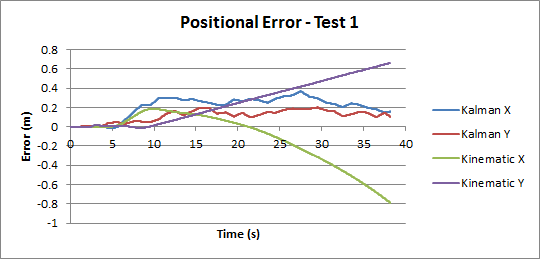
\includegraphics[width=\textwidth]{5-Testing/position_error_test_1.png}
\centering
\caption{Test 1: 25 degree right turn, 25 degree left turn, followed by long straight (from 9 seconds)}
\figlabel{posError1}
\end{figure}
\begin{figure}[ht]
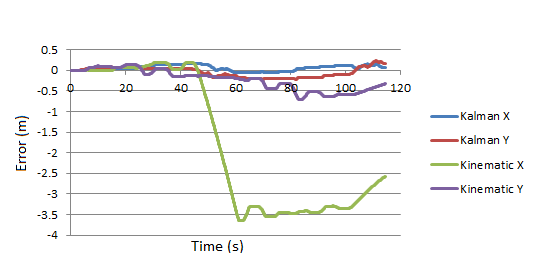
\includegraphics[width=\textwidth]{5-Testing/position_error_test_2.png}
\centering
\caption{Test 2: 2 x 90 degree right, long straight, 2 x 90 degree left, long straight} \figlabel{posError2}
\end{figure}

\subsection{Wheel encoder}
\seclabel{testingwheelencoder}
One of the primary functions of the wheel encoder was to give an accurate value for the distance travelled by the quad bike. To test the encoder, data was compared with values obtained from the display unit on the quad bike. The two data sets are overlaid in \figref{encoder20x} and the instantaneous difference shown. Some sampling was necessary to reduce the noise present in the encoder data. 20x was found to be the best as it was able to smooth the noise while keeping accurate to the display speed. It was clear that the wheel encoder was doing an adequate job of representing the display speed. The second test was to evaluate how accurate the speed represented the actual distance travelled when integrated over time. \Tabref{encoderIntegration} shows the results of three tests. Test 1 and 2 consisted of manually spinning 10 revolutions of the quad bike wheel on its stand at a consistent speed. Test 3 involved 3 complete stops of the wheel throughout the 10 revolutions.

\begin{figure}[ht]
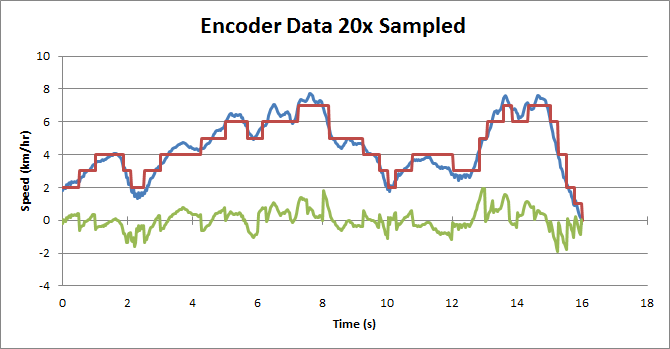
\includegraphics[width=1\textwidth]{5-Testing/encoder_data_20x_sampled.png}
\centering
\caption{Encoder speed reading compared with quad bike display with engine not running}
\figlabel{encoder20x}
\end{figure}

\begin{table}[ht]
\centering
\caption{Wheel encoder distance integration tests}
\label{encoderIntegration}
\begin{tabular}{l|l|l|l}
                                   & Test 1 & Test 2 & Test 3 \\ \hline
Rotations of the wheel:            & 10     & 10     & 10     \\
Number of readings:                & 7646   & 8843   & 19885  \\
Test time (seconds):               & 13.54  & 14.39  & 31.69  \\
Time interval (microseconds):      & 1770   & 1627   & 1594   \\
Circumference of wheel (m):        & 1.95   & 1.95   & 1.95   \\
Actual distance travelled (m):     & 19.5   & 19.5   & 19.5   \\
Calculated distance travelled (m): & 19.53  & 19.41  & 18.86  \\
\end{tabular}
\end{table}

\textcolor{red}{TALKING ABOUT LIVE TESTS WITH ENGINE RUNNING HERE}

\begin{figure}[ht]
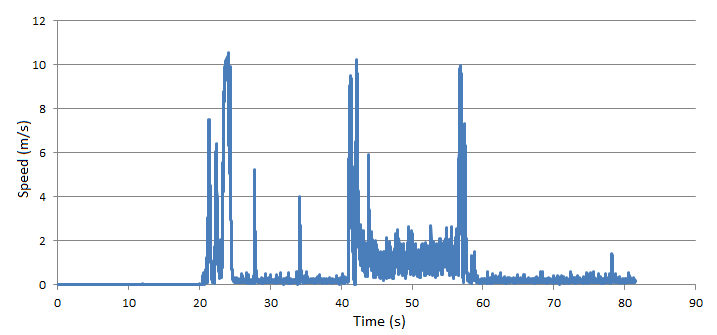
\includegraphics[width=1\textwidth]{5-Testing/Encoder_data_with_engine_running.png}
\centering
\caption{Encoder speed reading when stationary and engine off (0s - 20s), engine idling (20s - 40s), engine throttling (40s - 60s), and while supporting the encoder bracket (60s - 80s)}
\figlabel{encoderEngine}
\end{figure}

\subsection{Integrated positioning system}

\section{Quad bike systems testing}
Preliminary testing of the quad bike subsystems were required to determine their working range, functionalities and integration. The systems tested were the brakes, steering, throttle, gear selector, wheel encoder, and positioning system. Additional safety systems were also tested to ensure they functioned as intended.
The relevant test cases were documented in separate files (\textcolor{red}{REFER TO APPENDIX??}).

\subsection{Brake testing}
The brakes were required to control the quad bike speed as well as to bring the platform to a complete stop when commanded or in the case of an emergency. This requires accurate knowledge of the brake position for the varying brake intensities. The maximum brake intensity was chosen as the point where the wheels were unable to be turned by hand. This was found through small 5 percent increments in the actuator extension until the wheels were unable to rotate. The time required for the brake actuator to go from nill brake to maximum was \textcolor{red}{MEASURED TO BE 3 SECONDS}. This coupled with a reduction in throttle would ensure that the quad bike is able to stop in the required distance of 60cm as specified in the constraints. \textcolor{red}{THIS LAST SENTENCE IS THE ACTUAL TEST THAT WE NEED TO DO - NOT COMPLETE YET}

\subsection{Gear testing}
The ability to control what gear the quad bike is in was essential to the control and navigation of the project. 36 testing cases were identified for the gear actuator setup. The actuator could lie in one of nine possible positions which were identified based on the system set-up and had three final positions, reverse, neutral and forwards as well as a null option for no actuator movement. \figref{gearTruthTable} shows the final truth table.

\textcolor{red}{TABLE HERE}

The truth table indicates the gear selector code has full completion of the testing cases. The gear actuator should not move when the quad bike is in motion or when the throttle is engaged. This is to ensure that   A check in the software was implemented to achieve this. \textcolor{red}{DO WE NEED MORE ON THIS?}

\subsection{Steering testing}
The steering of the quad bike was achieved through the use of a stepper motor. Upon power up, the position of the wheels would be the zero position and movement to the left or right dictated by the angle sent to the stepper motor. From the user manual for the quad bike the lock out angle for the steering was \textcolor{red}{24 degrees NEED TO CHECK}, a limit for the steering angle was placed at 23 degrees to ensure no structural damage occurred. 

Initial tests found that when the quad bike was on the support stand with the wheels free, the steering behaved as expected. However, when a resistive load was applied in the direction of the steering angle, the stepper motor would stop and reset. This would result in a incomplete steering angle as well as a new off centre zero position being selected by the stepper motor.  It was found that the required power for the stepper motor to operate to the required torque was 440W whereas the power supply in the quad bike was only able to supply 44W. Replacement of the power supply with one of the correct power requirements resulted in steering angle control under operational loads.

The accurate turning radius for the platform was required for the navigation software. The quad bike was allowed to travel forward from a marked position with the steering at full lock. Once a full circle was complete, the quad bike was turned off. The turn radius was measured to be 2.7m. This was within the turning circle range decided upon in the navigation software.

\textcolor{red}{steering tests more?}

\subsection{Throttle testing}
The throttle is controlled via a rotational servo. Initial approximation of the throttle travel had the servo with zero throttle and maximum throttle at servo positions 75 and 150 respectively. With the engine warmed up, incremental increases resulted in an actual throttle response range to be calculated. Due to the circular sweep of the servo arm and some cable play, the minimum throttle position before a throttle response was found to be 97 and a maximum throttle position of 110 was chosen for the servo. This number was chosen due to the wheel speed in both forwards and reverse gears varying due to gearing and so the maximum servo position would be required for cruise speed in both directions of motion. A higher servo position than this would never be required for the chosen operating scenario.

\section{Navigation testing}
\subsection{Virtual platform navigation}
\subsection{Live navigation}
The virtual platform tests the functionality of the developed software program using the state values derived from initial testing. The software program for navigation were then transferred to the quad bike for actual system testing. (\textcolor{red}{REFER TO APPENDIX??})

\section{Integrated system testing}

\end{document}